\documentclass[a4paper, 12pt, mla]{homework}

\title[Genre Analysis of `None-Core Gameplay Ads']{Decoding the Deception: \\[0.1\baselineskip] Genre Analysis of `None-Core Gameplay Ads'}
\subtitle{ENGL 101-011\ \ First-Year Composition \linebreak Project 3: Analysis of a Genre}
\author{En-Chi (William) Lee}
\authorline{Originally submitted on November 17, 2023}
\mail{williameclee@arizona.edu}

\graphicspath{{./Figures/}}

\usepackage[scale=0.85]{FiraMono}
\usepackage{Alegreya, AlegreyaSans}

\definecolor{sandgreen}{RGB}{080, 130, 100}
\definecolor{brown}{RGB}{200, 175, 135}

\begin{document}
\maketitle

\noindent
After an exhaustive day at school, I turned to YouTube for relaxation while my dinner rotated in the microwave. 
My calm was, however, soon shattered by a loud mobile game advertisement (see \figref{FIG:HS-PtP}). 
A scene unfolded with a man in distress frantically fleeing from flames. 
An animated finger manipulated colossal sewing pins to remove obstacles along his escape. 
In a critical moment, the finger's aid failed, leading to the man's demise in the flames.

\begin{figure}[htb]\centering
	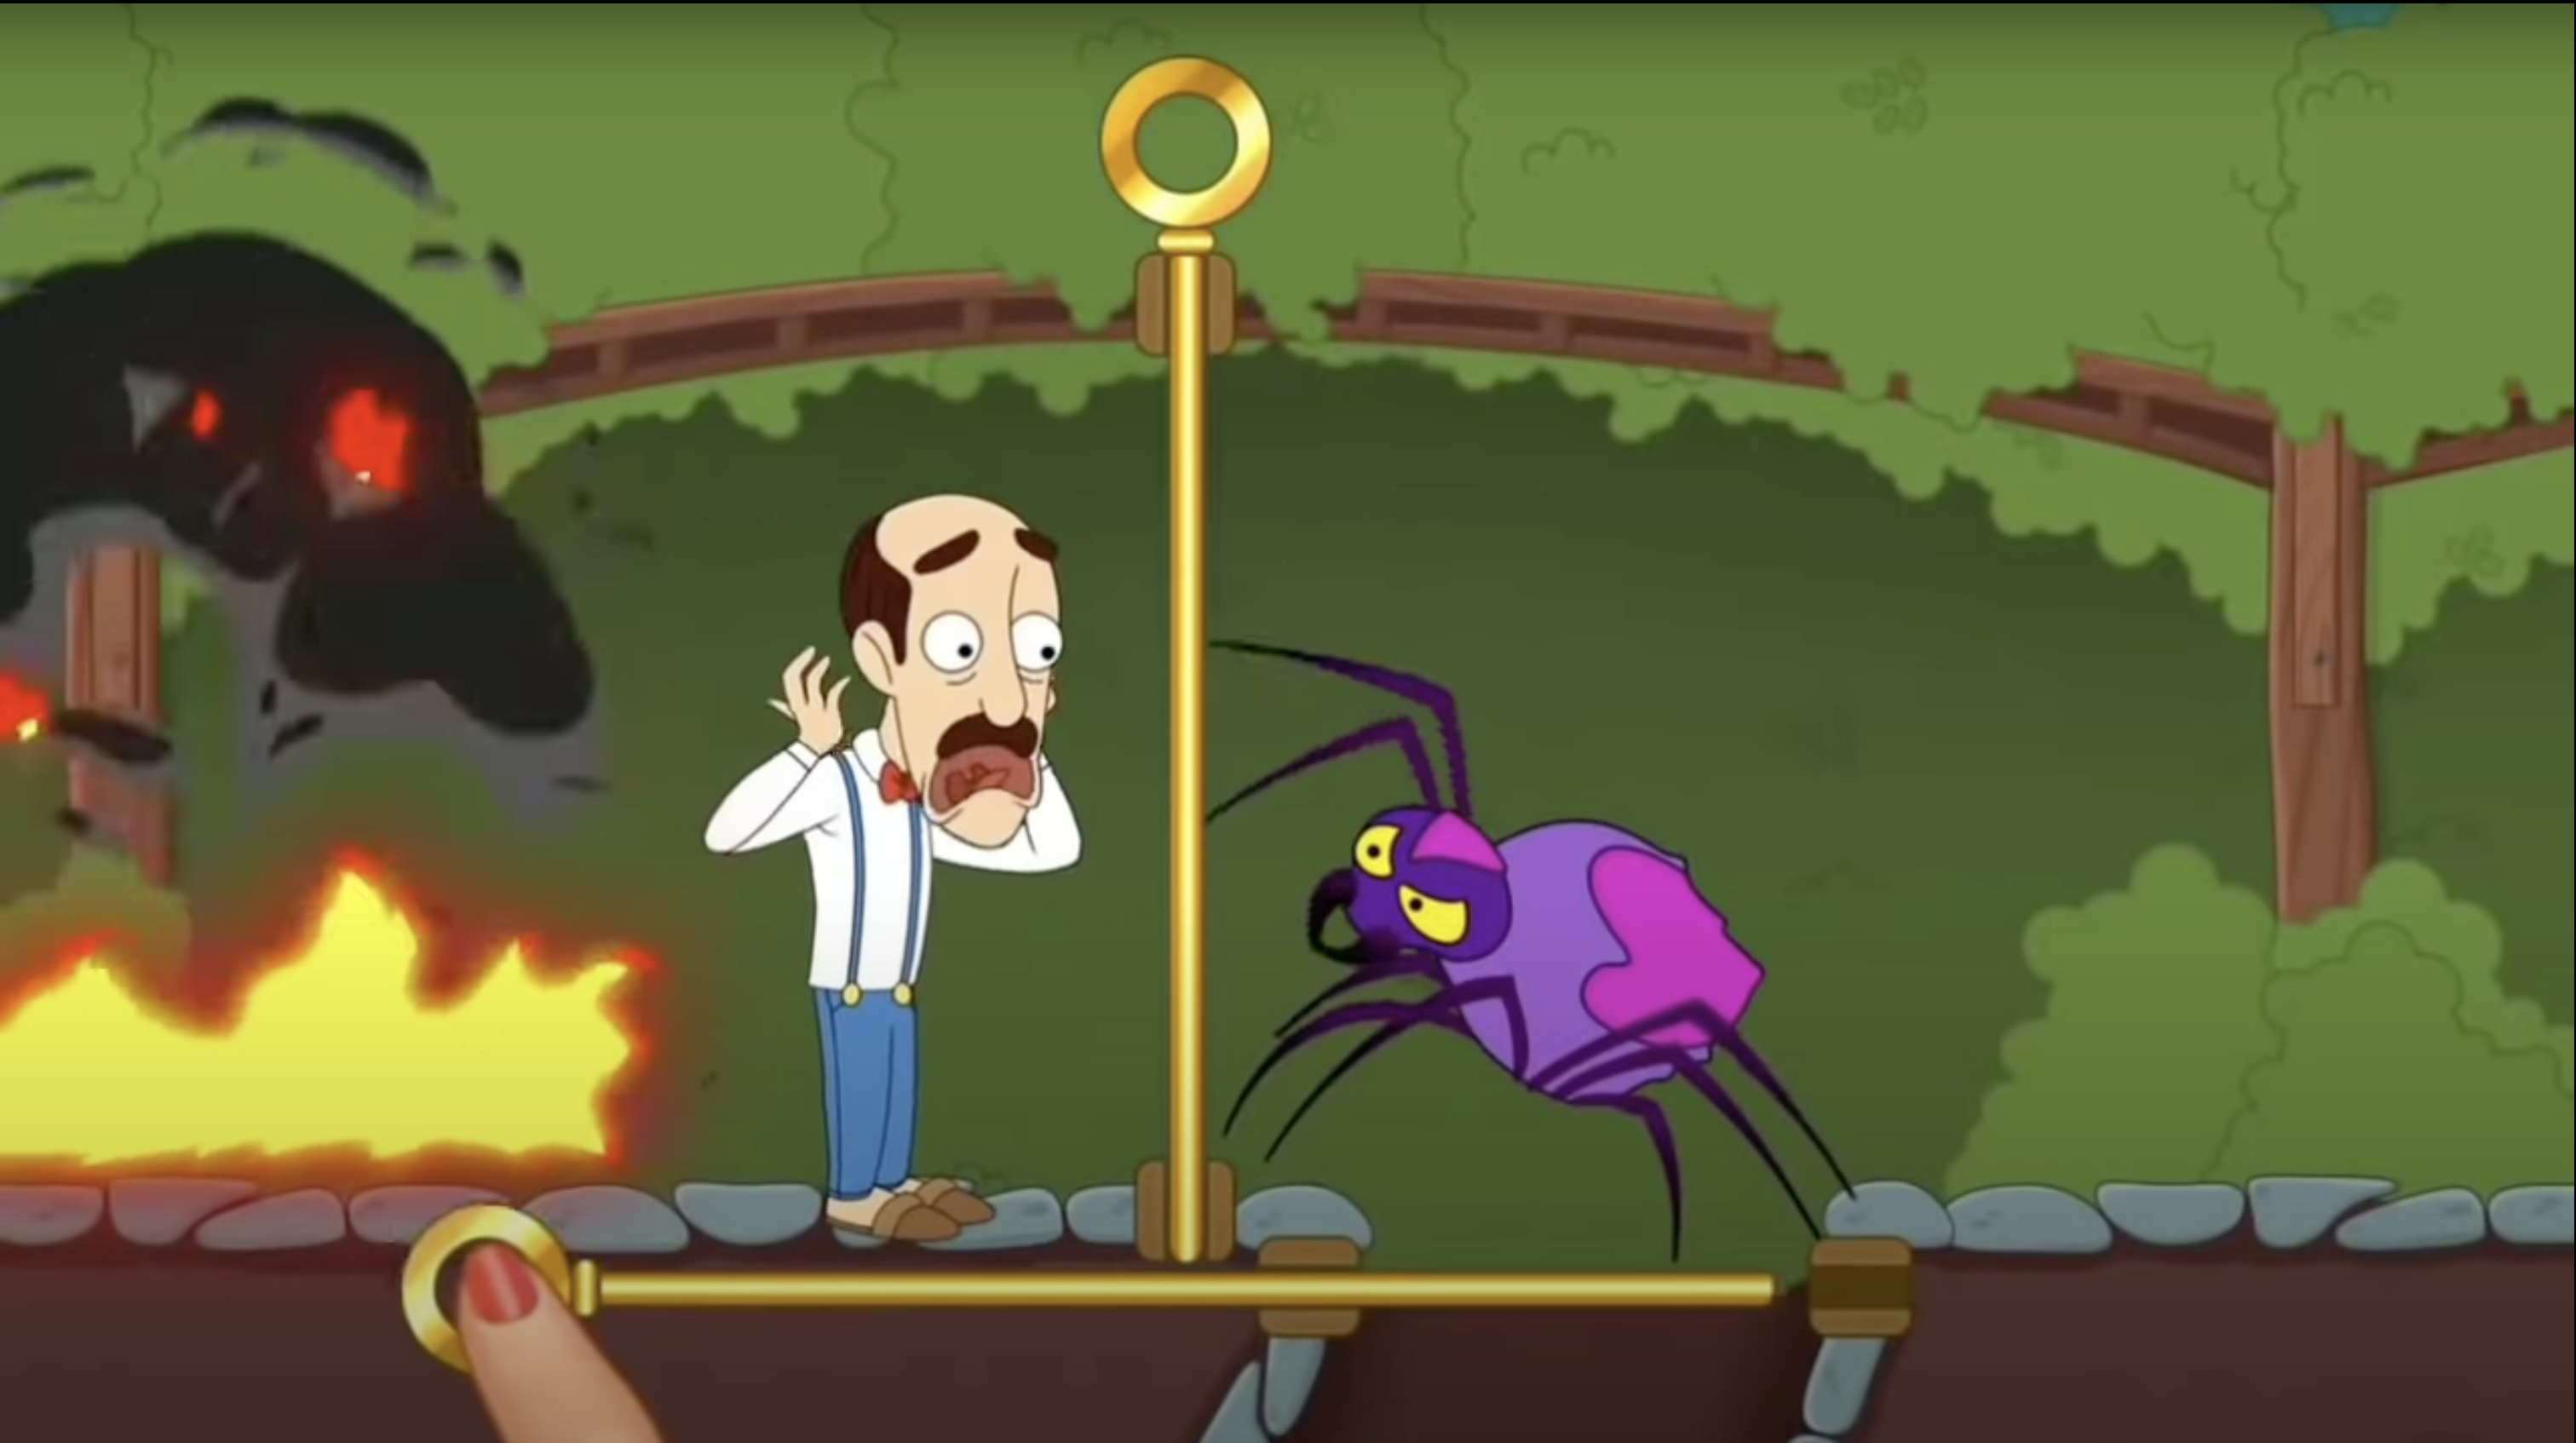
\includegraphics[width=0.9\linewidth]{Homescapes-Spider.png}
	\captionsetup{width=0.9\linewidth}
	\caption{A screenshot of a \textit{Homescapes} non-core gameplay ad on YouTube. \protect\cite{DG:Homescapes, YT:Homescapes-Spider}}
	\label{FIG:HS-PtP}
\end{figure}

The drama concluded by displaying the game's title, \textit{Homescapes}, alongside an `Install Now' button \cite{DG:Homescapes}. 
While intuitively suspicious about the commercial's authenticity---a result of encounters with numerous similar ads---its absurdity piqued my curiosity. 
I downloaded the game, only to be greeted by chores of redecorating a mansion, a far cry from the thrilling escapade portrayed.

This stark discrepancy showcased the deceptive allure of `non-core gameplay ads'. 
Despite widespread awareness of their deviation from actual gameplay, these ads effectively draw viewers with exaggerated narratives.

\section*{What Constitutes `Non-Core Gameplay Ads'?}
The \textit{Homescapes} advertisement exemplifies a distinct subgenre in mobile game advertising characterised by its use of animated sequences that simulate gameplay experiences. 
Notably, these depictions often significantly deviate from the actual game mechanics. 
Although this advertising approach raises ethical questions, it does not always constitute false advertising. 
The gameplay elements shown in these ads exist within the games, yet they are not the principal aspect of the gaming experience \cite{WB:Semenov2023}. 
This type of promotional content has been accurately described as `non-core gameplay (NCG) ads' by \citeA{BF:Nexters2023}.
In this analysis, `NCG ads' are defined as commercials that: 
\begin{enumerate} 
	\item Promote a mobile game; 
	\item Utilise primarily animation-based footage to simulate gameplay mechanics; 
	\item Do not feature live actors or celebrities for voiceovers or promotional roles.
\end{enumerate}

Although created by various game developers, NCG advertisements share a distinct aesthetic that cements their place as a unique subgenre in digital game advertising. 
An animated finger is a recurring feature in these ads, implying player engagement with the game (as seen in \figref{FIG:HS-PtP,FIG:PM-Puzzle,FIG:HW-Puzzle}). 
The gameplay showcased typically comprises straightforward, self-contained mini-puzzles designed to be intuitively understood by viewers.

\begin{figure}[bt]\centering
	\begin{subfigure}[t]{0.3\linewidth}\centering
		
\includegraphics[width=\linewidth]{PM-Drama.png}
		\caption{A provoking scene}
		\label{FIG:PM-Drama}
	\end{subfigure}
	\begin{subfigure}[t]{0.3\linewidth}\centering
		
\includegraphics[width=\linewidth]{PM-Puzzle.png}
		\caption{Mini puzzles}
		\label{FIG:PM-Puzzle}
	\end{subfigure}
	\begin{subfigure}[t]{0.3\linewidth}\centering
		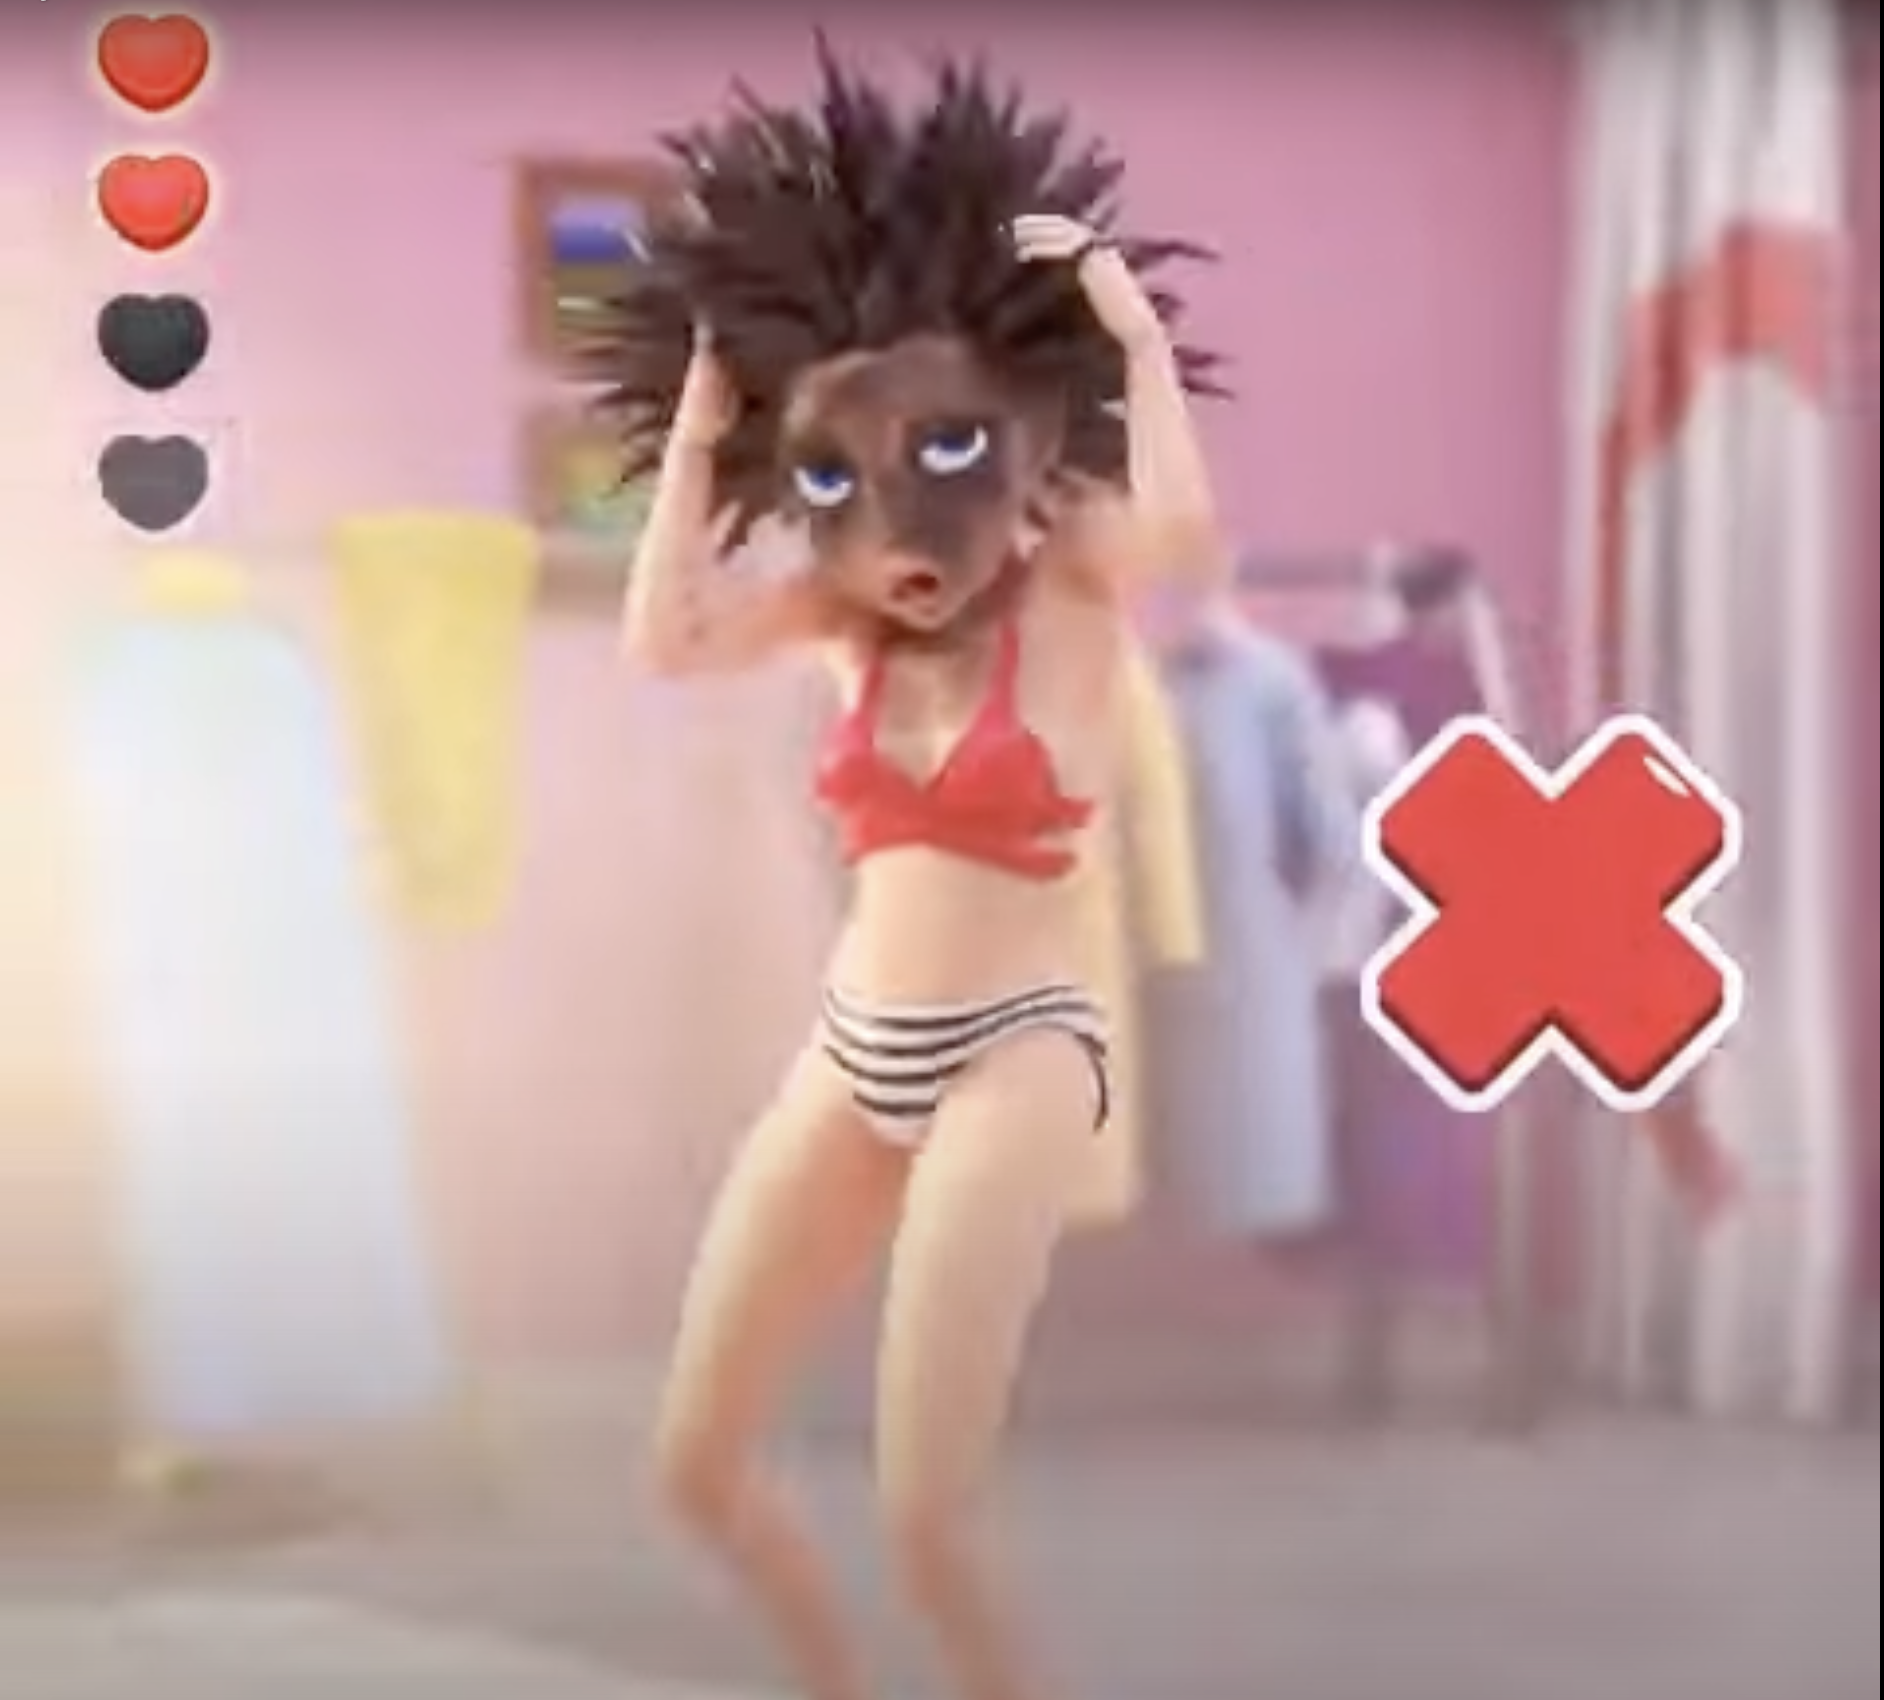
\includegraphics[width=\linewidth]{PM-Fail.png}
		\caption{Outcome of failed puzzle attempt}
		\label{FIG:PM-Fail}
	\end{subfigure}
	\captionsetup{width=0.92\linewidth}
	\caption{Screenshots of a \textit{Project Makeover} commercial on YouTube demonstrating a classic non-core gameplay ad format \protect\cite{DG:ProjectMakeover, YT:ProjectMakeover-Mud}}
	\label{FIG:PM}
\end{figure}

The narrative structure of NCG ads is also remarkably uniform and predictable. 
A representative case is the \textit{Project Makeover} commercial (\figref{FIG:PM}) \cite{DG:ProjectMakeover, YT:ProjectMakeover-Mud}. 
It begins with a mud-soaked girl discovering her partner's unfaithfulness (\figref{FIG:PM-Drama}). Interactive elements emerge (\figref{FIG:PM-Puzzle}), with an animated finger making choices that lead to fleeting success or ultimate failure (\figref{FIG:PM-Fail}).

In contrast, the \textit{Hero Wars} promotional video (\figref{FIG:HW}) \cite{DG:HeroWars,YT:HeroWars-Legend} echoes this structure: a central character faces challenges, and despite the player's attempts at puzzle-solving, the outcome is typically unsuccessful.
This pattern is consistent across various NCG ads, including the previously mentioned \textit{Homescapes} ad. 
A notable evolution in NCG ads has been the increase in the absurdity of their plotlines, yet this foundational narrative structure has remained unchanged since its debut.

\begin{figure}[bt]\centering
	\begin{subfigure}[t]{0.3\linewidth}\centering
		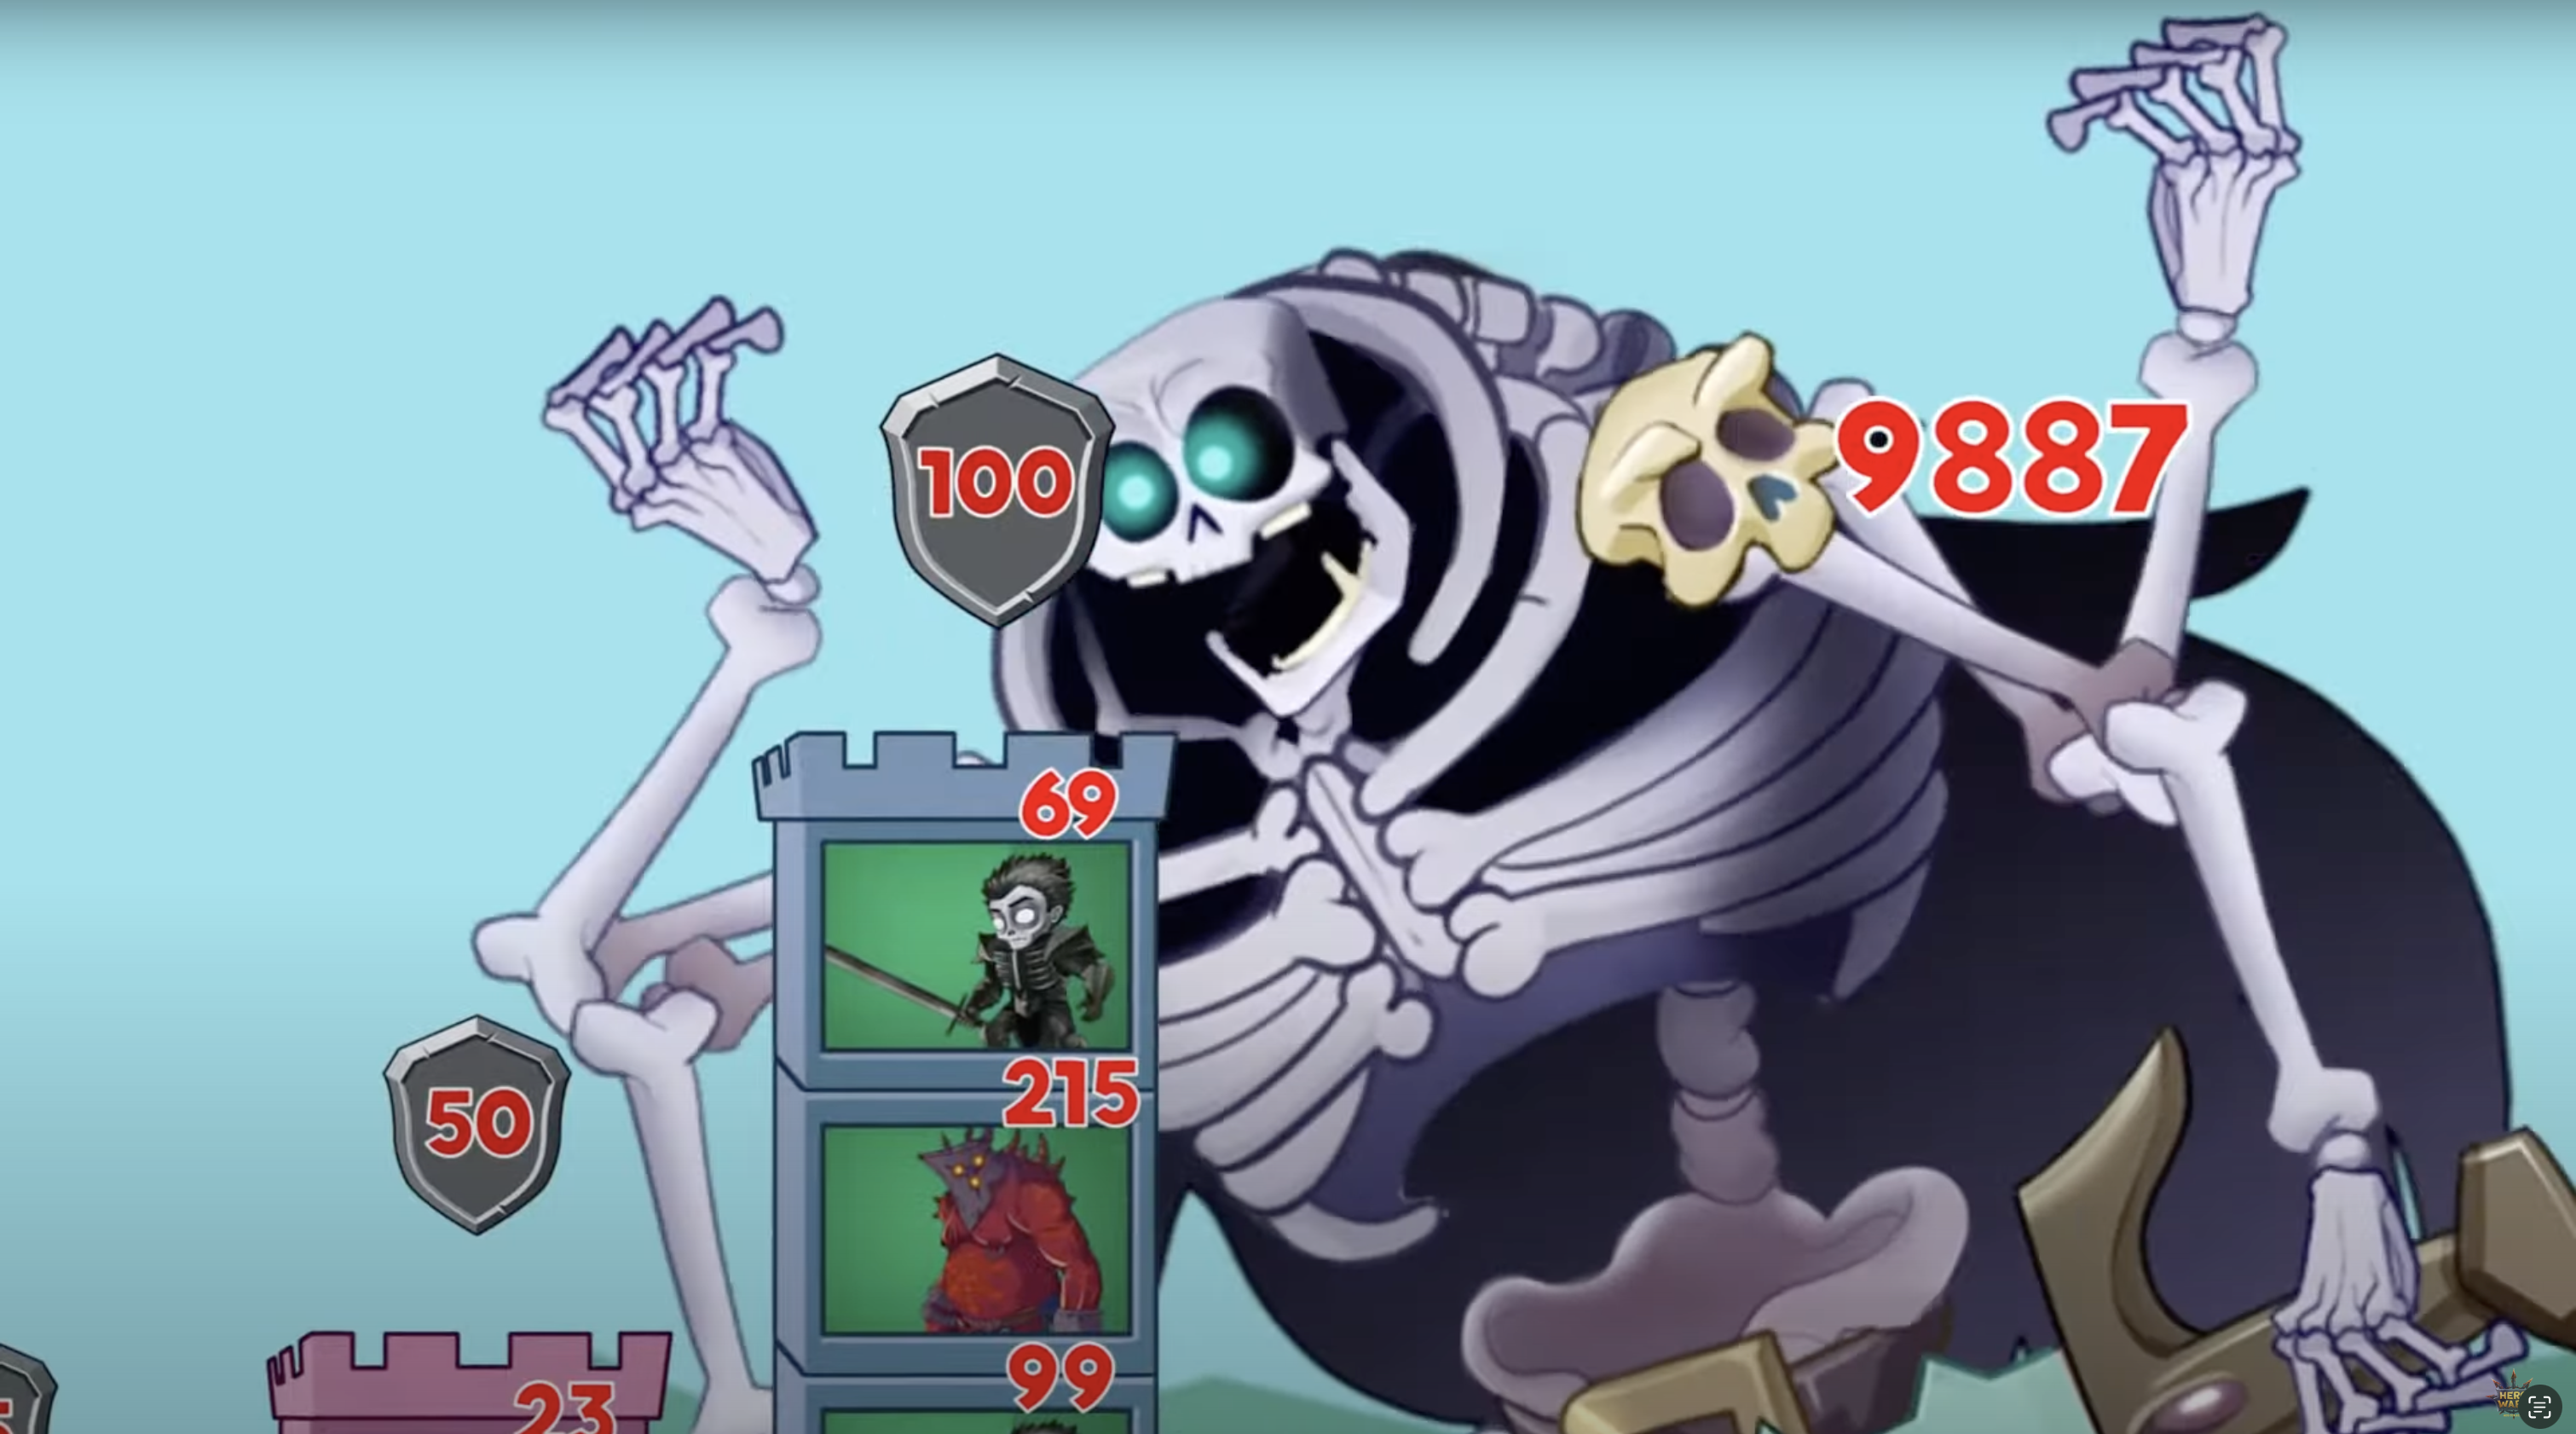
\includegraphics[width=\linewidth]{HW-Drama.png}
		\caption{A challenge}
		\label{FIG:HW-Drama}
	\end{subfigure}
	\begin{subfigure}[t]{0.3\linewidth}\centering
		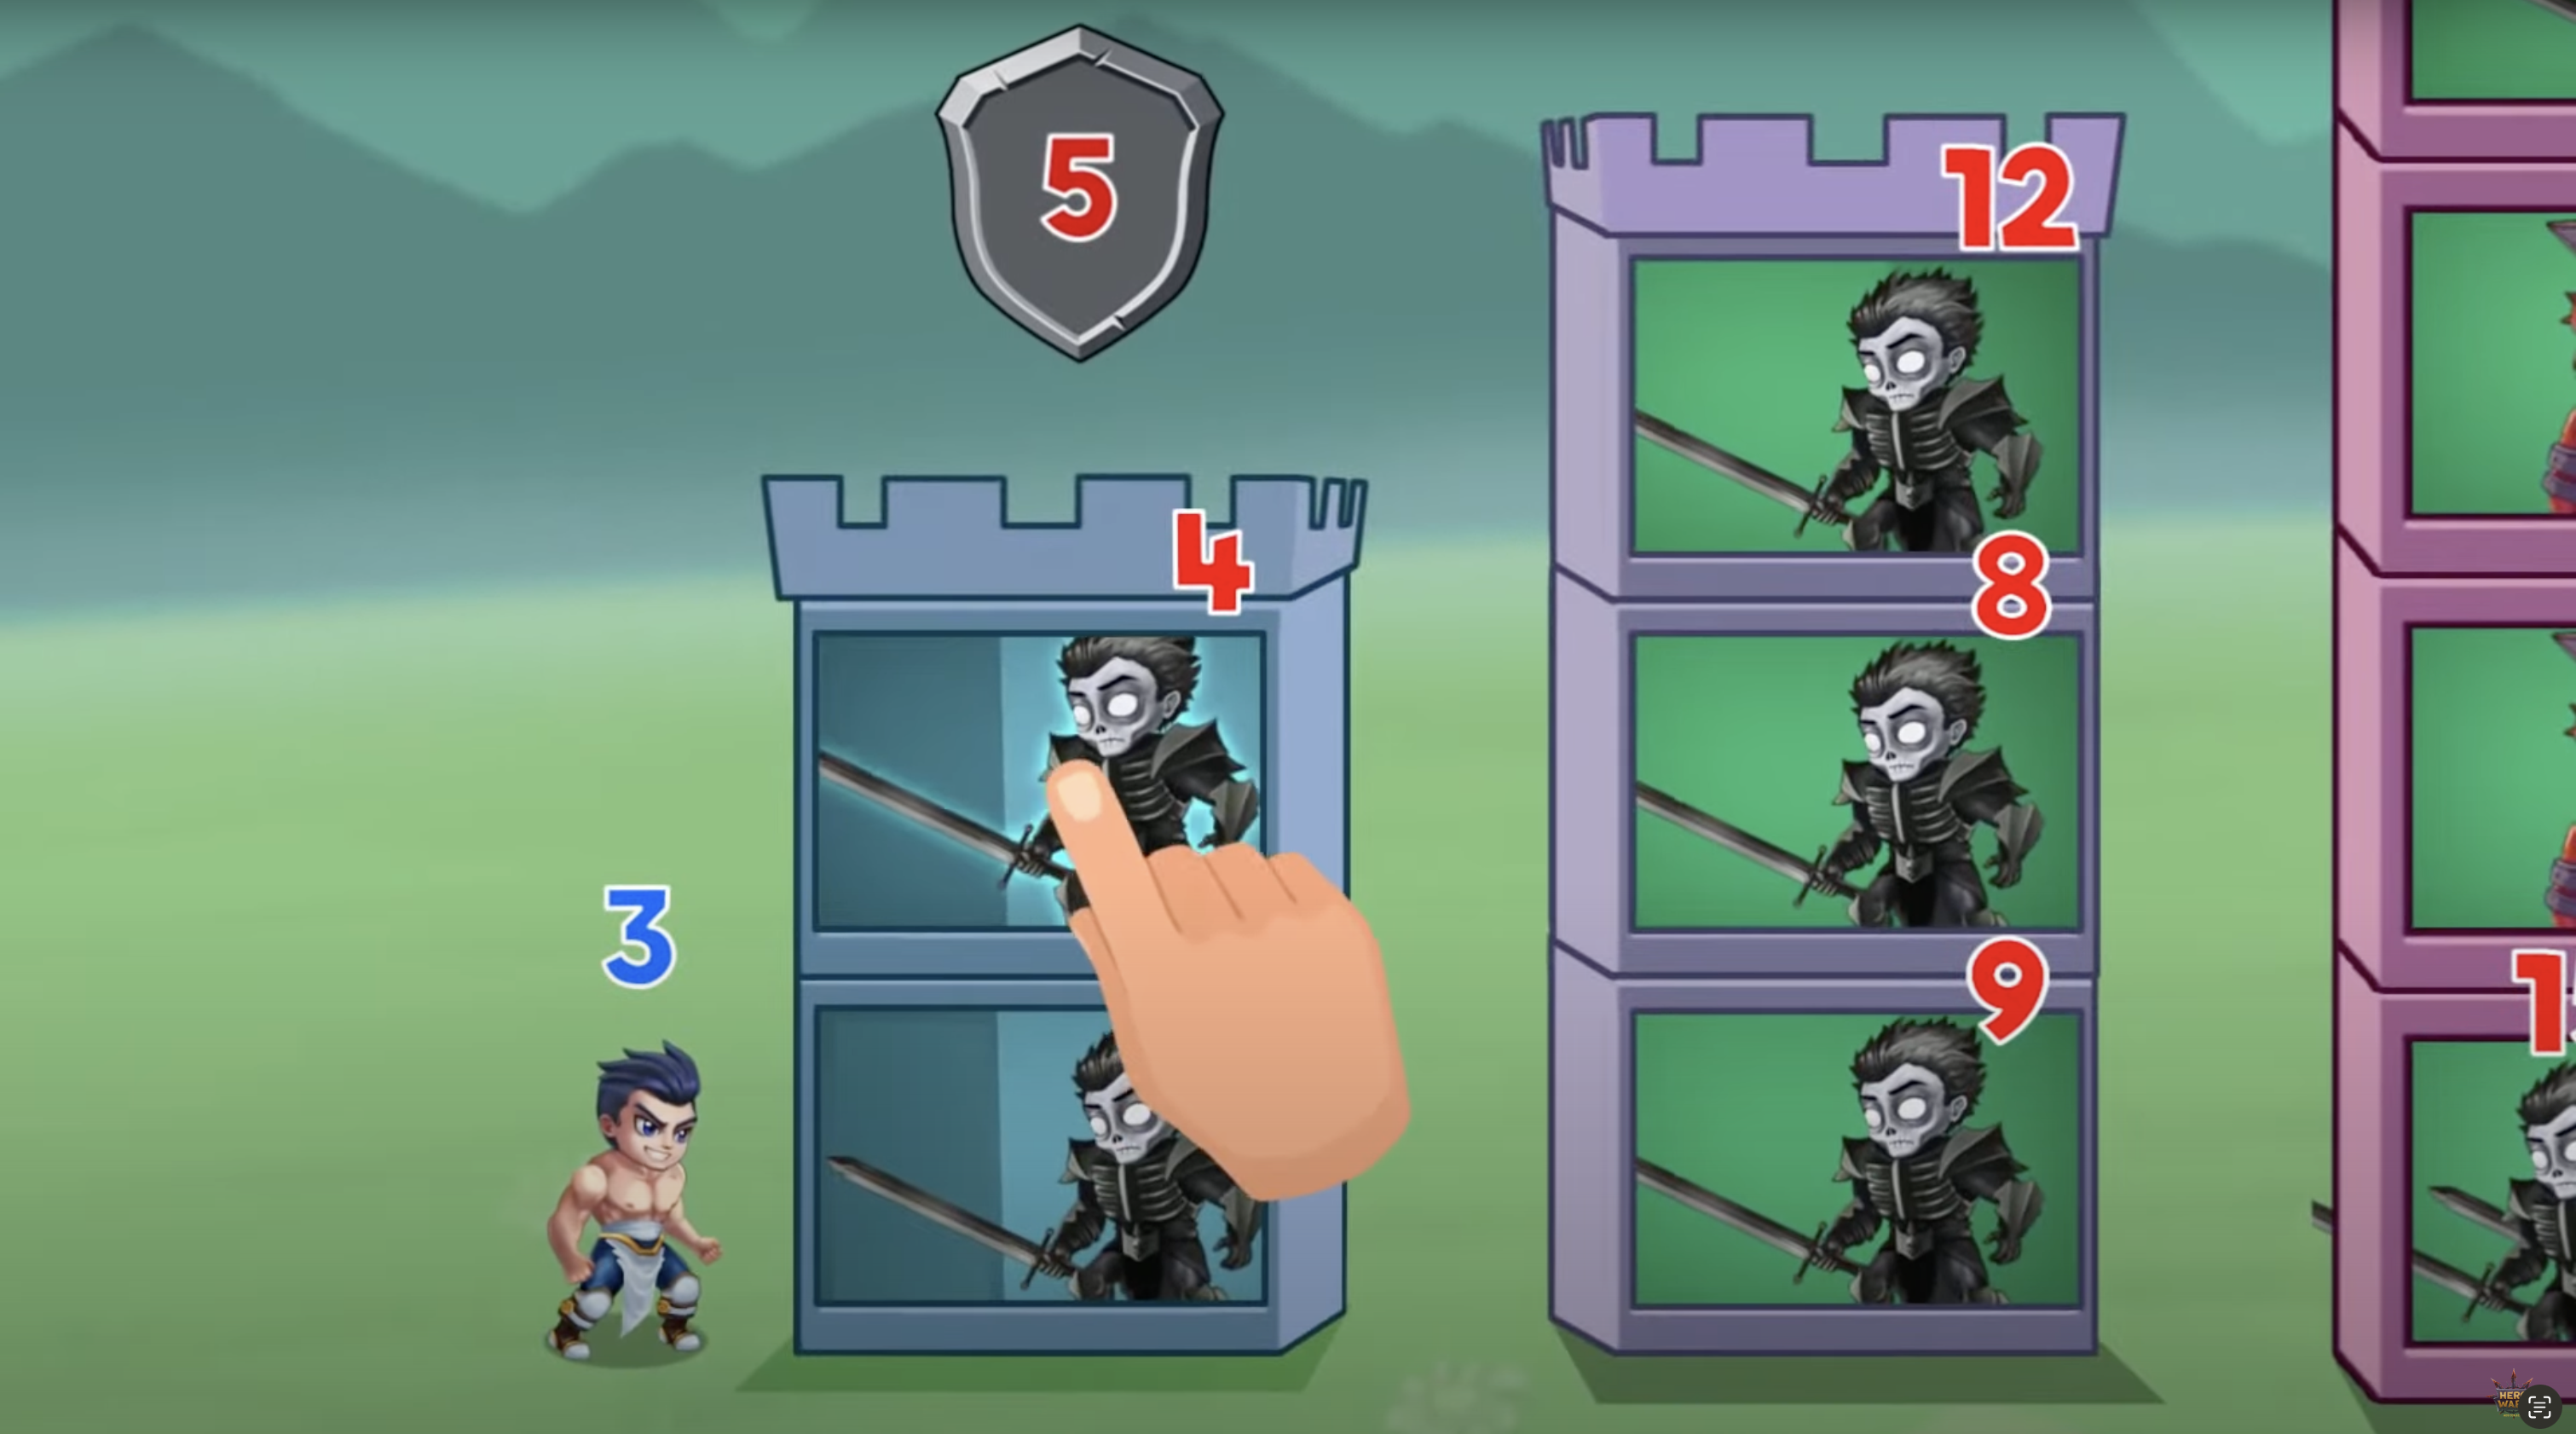
\includegraphics[width=\linewidth]{HW-Puzzle.png}
		\caption{Simple mini puzzles}
		\label{FIG:HW-Puzzle}
	\end{subfigure}
	\begin{subfigure}[t]{0.3\linewidth}\centering
		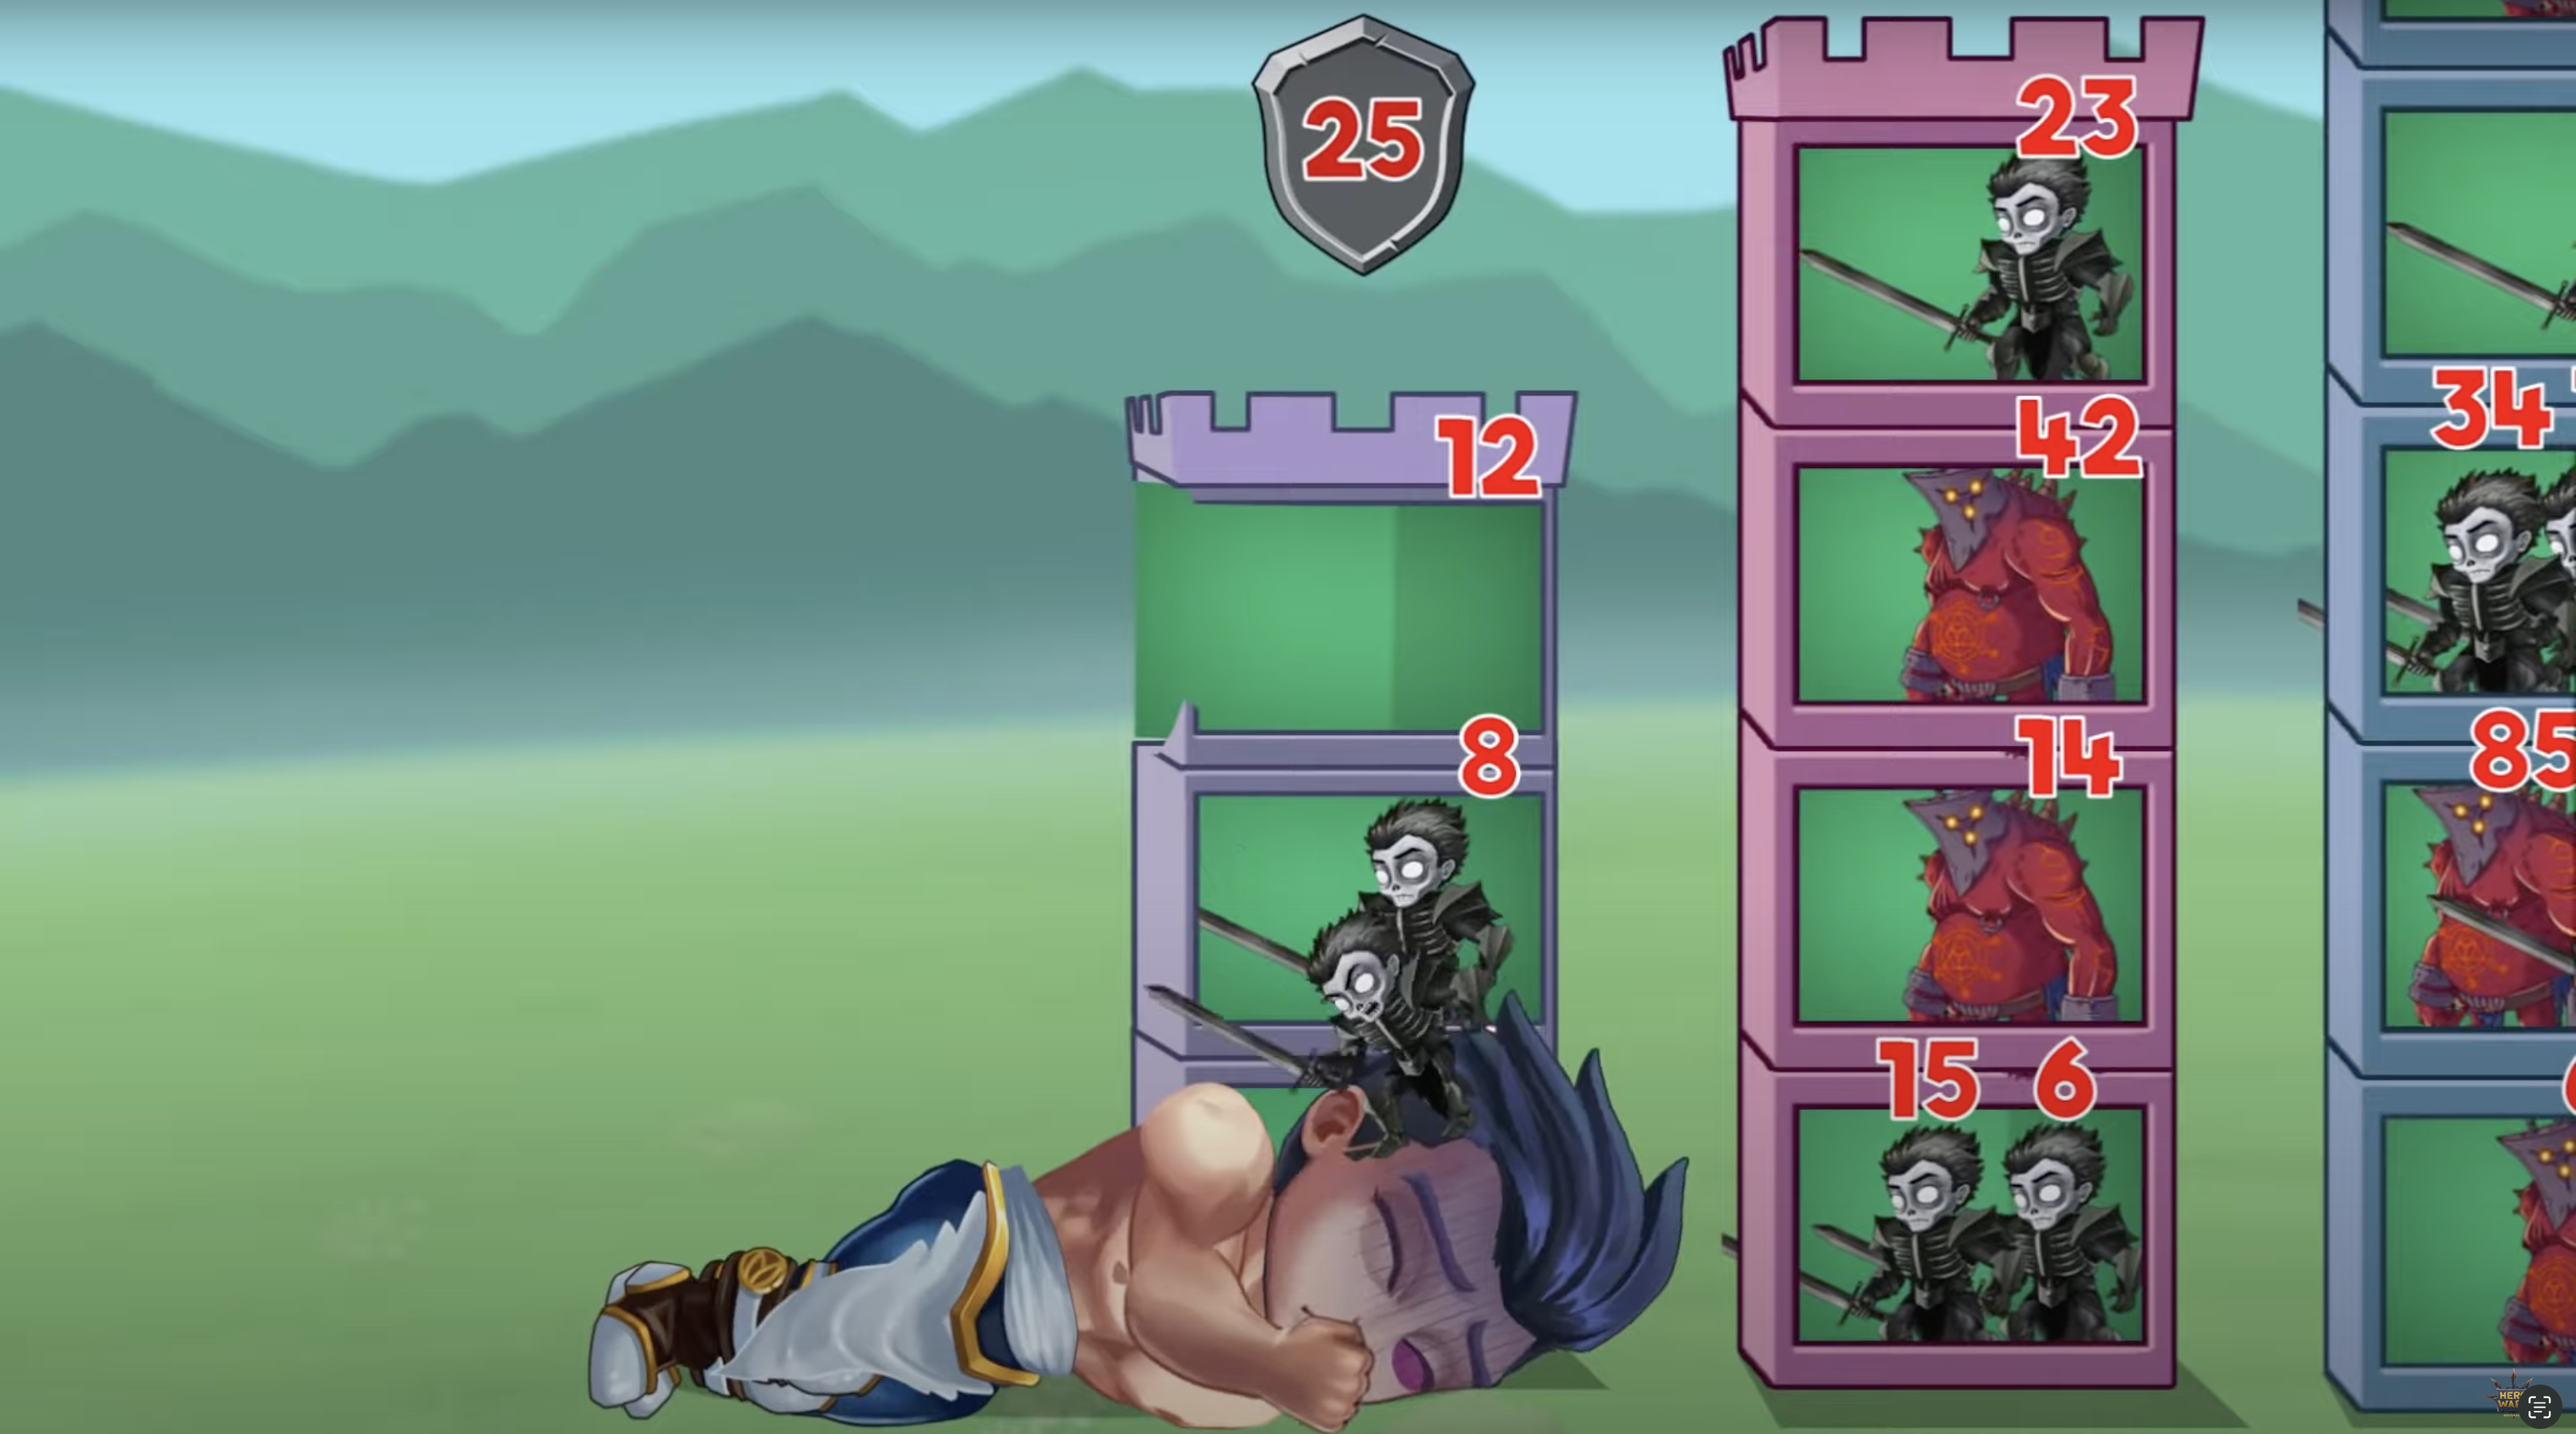
\includegraphics[width=\linewidth]{HW-Fail.png}
		\caption{Unsuccessful puzzle attempt}
		\label{FIG:HW-Fail}
	\end{subfigure}
	\captionsetup{width=0.92\linewidth}
	\caption{A \textit{Hero Wars} commercial on YouTube illustrating a classic non-core gameplay ad format \protect\cite{DG:HeroWars, YT:HeroWars-Legend}}
	\label{FIG:HW}
\end{figure}


\section*{The Power of Emotion: What Drives the Popularity of Non-Core Gameplay Ads?} 
NCG advertisements predominantly promote `casual mobile games', characterised by their simple rules and low time commitments. 
In this game genre, game companies' revenue models centre on in-game purchases and the integration of additional advertisements, turning players into commodities \cite{BK:Nieborg2017}.

Consequently, the core objective of these commercials is to captivate viewers and stimulate game downloads, a goal at which they have been notably successful. 
\citeA{RA:Mago2020} traces the emergence of this genre to the summer of 2019, noting \textit{Homescapes} and \textit{Hero Wars} as earliest perpetrators \cite{DG:Homescapes, DG:HeroWars}. 
The immediate success has led many marketing teams to adopt similar advertising tactics. Over the last four years, this approach has become a standard in NCG advertising.

The primary audience for these advertisements encompasses a broad internet community, but `casual gamers' form the central focus \cite{WB:Knezovic2023}. 
This group `play to pass the time and simply want to be entertained and have some fun during a break' and is particularly drawn to the accessible nature of mobile gaming, which starkly contrasts the more demanding financial and time commitments associated with traditional console gaming.

While rarely mirroring the actual gameplay, the puzzles portrayed in NCG advertisements successfully communicate a sense of effortless, enjoyable escapism \cite{WB:Knezovic2023}. 
\citeA{RA:Ihsan2022} points out that the ease and low stakes of accessing free mobile games make emotional appeals in ads more compelling than logical arguments (see \figref{FIG:EmotionalAppeals}). 
As a result, these commercials often employ dramatic narratives and emotionally charged scenarios to prompt impulsive downloads. 
They evoke empathy or guilt by depicting protagonists in distress and a sense of challenge through the apparent failure to solve simple puzzles.

\begin{figure}[htb]\centering
	\def\bwidth{0.4}
\newcommand{\drawbar}[5]{
	\filldraw[#5,thick] (0,{-#3+\bwidth}) -- (0,{-#3-\bwidth}) node[midway,anchor=east]{\sffamily #1} -- (#2,{-#3-\bwidth}) -- (#2,{-#3+\bwidth}) node[midway,anchor=west]{\sffamily #4} -- cycle;
}
\newcommand{\drawbars}[5]{
	\fill[#5] (0,{-#3+\bwidth}) -- (0,{-#3-\bwidth}) node[midway,anchor=east,align=right]{\sffamily #1} -- (#2,{-#3-\bwidth}) -- (#2,{-#3+\bwidth}) node[midway,anchor=west]{\sffamily#4} -- cycle;
}

\def\colourE{sandgreen}
\def\colourR{brown}

\begin{tikzpicture}[x=0.14cm,y=0.7cm]
	\drawbar{Emotional appeals}{79.69}{-1.5}{80\%}{fill=\colourE}
	\drawbars{Humour}{18.67}{2}{19\%}{\colourE}
	\drawbars{Adventure}{15.91}{4}{16\%}{\colourE}
	\drawbars{Joy, compassion, \\[-0.2\baselineskip]\sffamily \& love}{1.38}{7}{1\%}{\colourE}
	\drawbars{Sexual}{9.77}{6}{10\%}{\colourE}
	\drawbars{Guilt \& sadness}{18.17}{3}{18\%}{\colourE}
	\drawbars{Violence \& fear}{15.66}{5}{16\%}{\colourE}
	\drawbar{Rational appeals}{20.31}{-0.5}{20\%}{fill=\colourR}
	\drawbars{Product \\[-0.2\baselineskip]\sffamily features appeal}{19.55}{1}{20\%}{\colourR}
	\drawbars{Product/service \\[-0.2\baselineskip] \sffamily popularity}{0.63}{8}{1\%}{\colourR}
	\draw[dashed] (0,-0.25) -- (80,-0.25);
	\draw[very thick] (0,2) -- (0,-8.5);
\end{tikzpicture}
	\caption{Frequencies of different \textcolor{\colourE}{emotional} and \textcolor{\colourR}{rational} appeals used in 100 mobile game advertisements published on YouTube channels
	in 2017-2021 \protect\cite{RA:Ihsan2022}}
	\label{FIG:EmotionalAppeals}
\end{figure}


Additionally, some NCG ads, such as those for \textit{Project Makeover}, have introduced increasingly sexually suggestive storylines to stir strong emotional responses. 
In this context, how accurately these ads reflect the actual gameplay becomes secondary. 
The more memorable or contentious an advertisement is, the more likely it will lead to game downloads.
Moreover, by going beyond the core gameplay mechanics, NCG ads can incorporate other appealing game aspects, like narrative and resource management elements. 
This approach broadens their appeal, attracting players who might not initially be interested in the gameplay mechanics.

\section*{Public Perception of the Non-Core Gameplay Advertising Genre}
The NCG advertising approach, perfected by \textit{Hero Wars} and similar games, has markedly influenced player engagement in the casual mobile gaming genre. 
A survey by \citeA{BF:Nexters2023}, the company behind the game, underscores this impact. 
A considerable 71\% of American respondents have reported encountering NCG promotions, and many voiced dissatisfaction after downloading the games.

Prompted by the increasing discontent, a petition was initiated in August 2019, shortly after the emergence of these advertisements, gaining thirteen thousand signatures \cite{WB:Hughes2019}.
Mirroring the escalating concerns regarding the truthfulness of such advertisements, the UK's Advertising Standards Authority took action in 2020, labelling two commercials for \textit{Homescapes} and \textit{Gardenscapes} as 'not representative' \cite{WB:BBC2020,DG:Homescapes,DG:Gardenscapes}.

However, despite most players finding the actual gameplay less enthralling than depicted in the advertisements, half of those who downloaded the games based on these ads remained engaged with them, according to \citeA{BF:Nexters2023}. 
This contradictory response suggests that, while the initial misrepresentation might stain game ratings, they also establish a user base that eventually develops a liking for these games \cite{RA:Mago2020}.
There is a rising tolerance among players for such advertising tactics.

The widespread adoption of NCG advertising strategies has led to homogenisation within the casual mobile gaming market, with little effort invested in innovation. 
Many companies replicate successful formulas, such as the 'match-3' mechanics popularised by \textit{Candy Crush Saga} \cite{DG:CandyCrush}, which are prominent in games like \textit{Homescapes} and \textit{Royal Match} \cite{DG:RoyalMatch}. Consequently, these games resort to increasingly bold and sensational advertising methods to differentiate themselves in the highly competitive market.


\section*{The Cost of Indulgence in Non-Core Gameplay Advertising}
The emergence and widespread adoption of NCG advertisements mark a transition in the gaming industry's commercial practices, reflecting a transformation in how we, predominantly as casual gamers, interact with gaming content. 
The low-commitment nature of downloading free mobile games paves the way for decisions driven more by emotional influence than logical evaluation. 
With their increasingly fantastical and provocative narratives, NCG advertisements are meticulously crafted to stimulate strong reactions, capitalising on the audience's emotional susceptibility.
In this environment, where emotional resonance outweighs logical assessment, the accuracy of advertisements in depicting actual gameplay becomes irrelevant.
This situation has given rise to an implicit yet toxic understanding between marketing teams and their audience: we acknowledge the deceptive nature of these ads yet continue to download the games they promote. 

Nevertheless, this indulgence comes at a cost. 
We are normalising ethically questionable practices and contributing to the erosion of integrity and creativity in games and their advertising. 
This trend pushes the industry towards a future where emotional persuasion overshadows authenticity and innovative content.


\vfill
\setstretch{1.2}
\bibliography{bibliography-ENGL101_gamePlayAds.bib}


\end{document}